\label{sec:exp}

\section{Setup}
\label{sec:exp_setup}
\paragraph{Benchmark.} We evaluate on \textbf{35 identities $\times$ 40 pose
prompts $=1400$ generations}. The 35 reference identities
(Fig.~\ref{fig:idgallery}) span a wide range of age, gender, and ethnicity; every
method receives the \emph{same single} reference per identity (one-shot) and the
identical prompt set. The 40 prompts share a fixed template whose \emph{pose}
slots are the controlled variable, tiling the
$2\,(\text{yaw})\!\times\!2\,(\text{over-the-shoulder})\!\times\!2\,(\text{chin})=8$
pose cells with five demographic/scene variants each (Tab.~\ref{tab:prompts}), so
pose is measured on a balanced grid while scene and demographic vary for
diversity. Rotate-ID generates with FLUX.2-klein at $1024^2$, four steps, fixed
seed.
% --- ID gallery (figures/make_id_gallery.py from SoftREPA/ID_image_35) ---
\begin{figure}[t]\centering
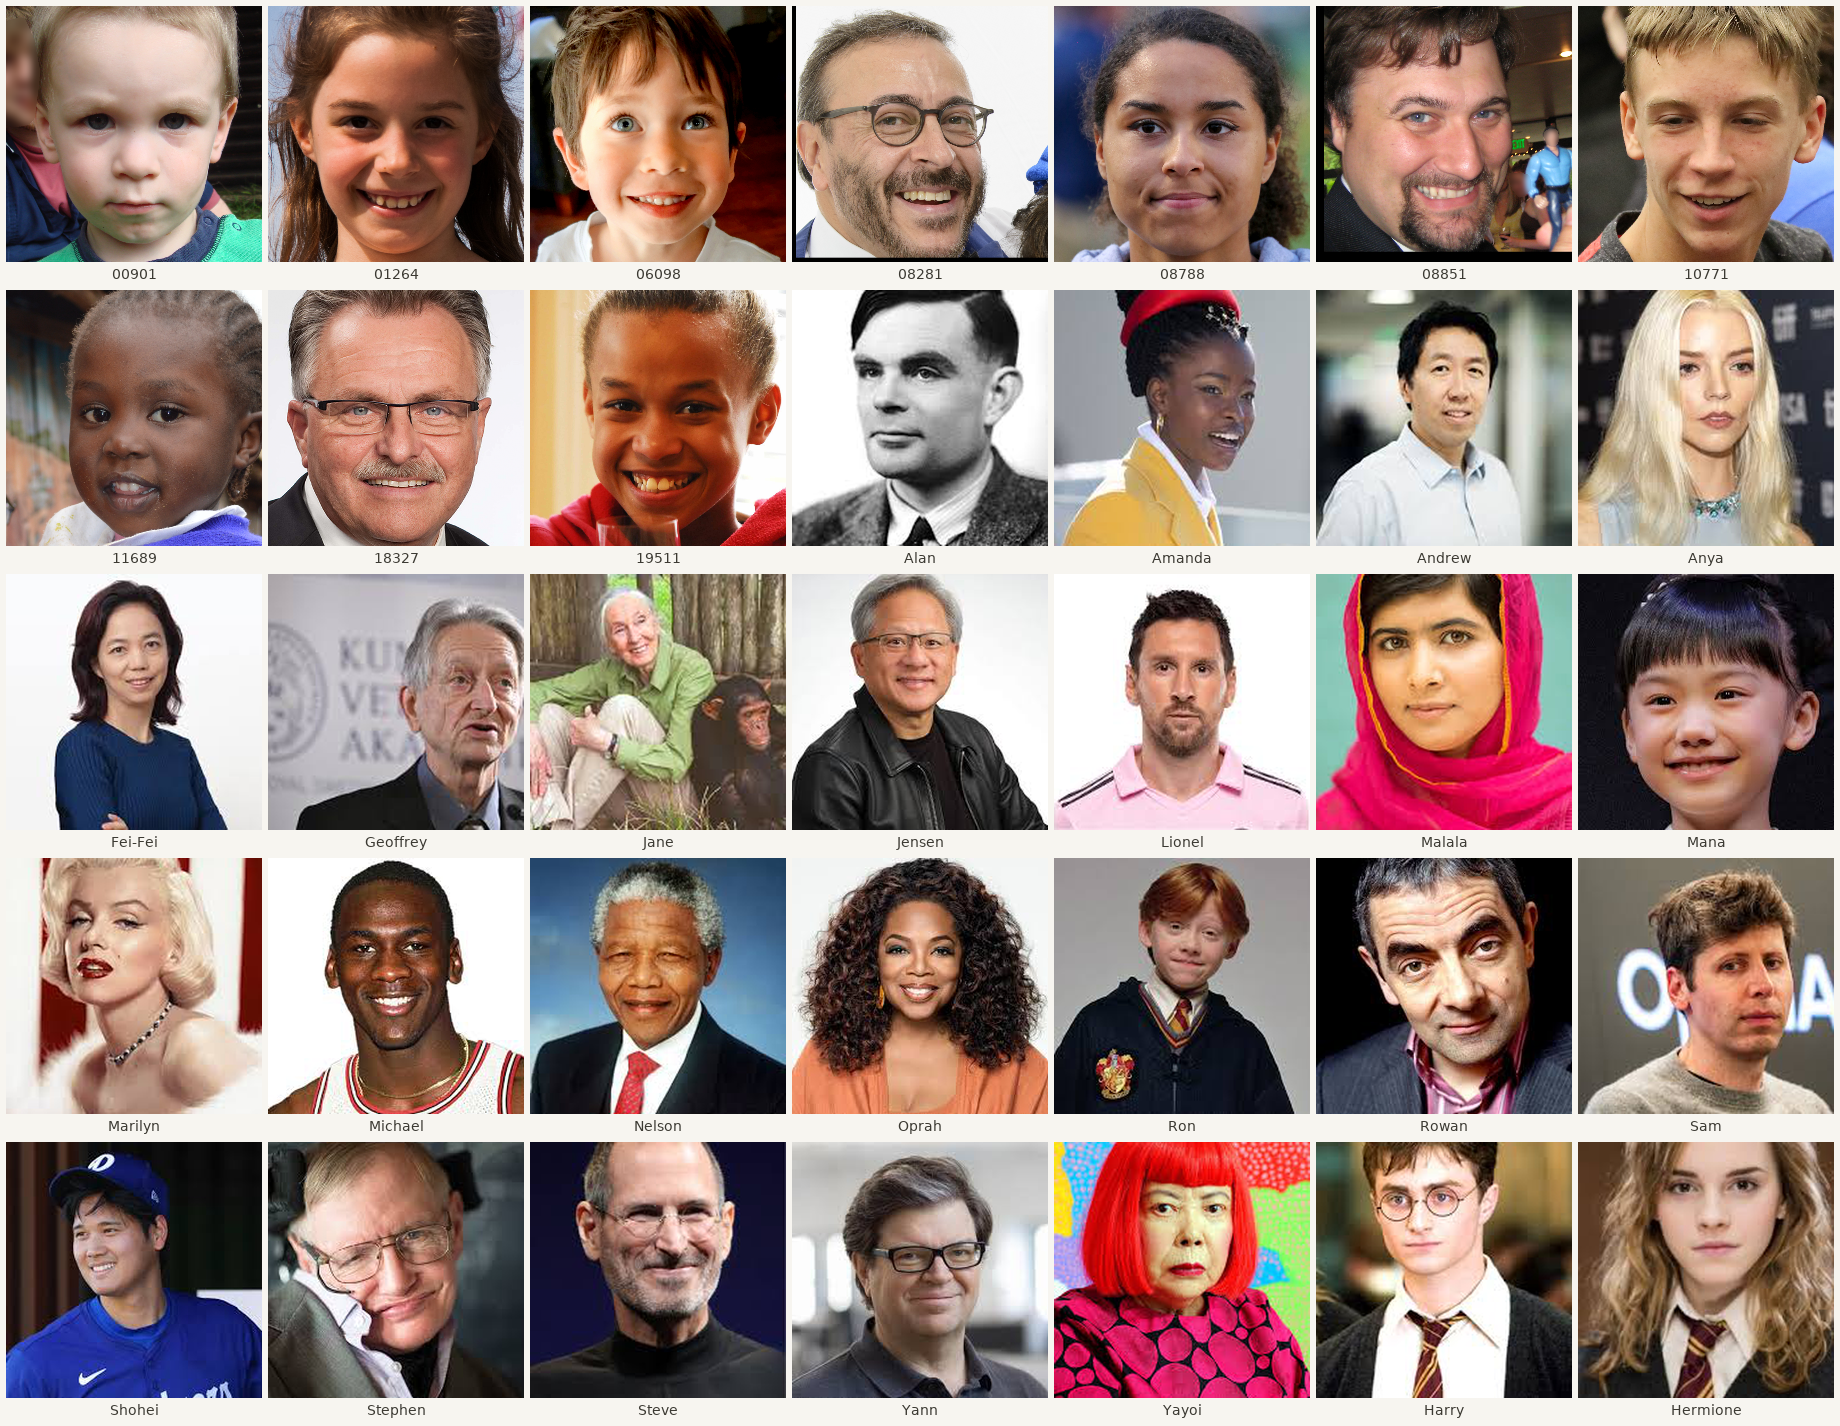
\includegraphics[width=0.6\linewidth]{figures/id_gallery.png}
\caption[The 35 reference identities (one-shot inputs)]{\textbf{The 35 reference identities (one-shot inputs).} Every method
receives exactly \emph{one} of these images per identity. The set spans a wide
demographic range (age, gender, ethnicity) and head-pose/expression of the
reference, mixing FFHQ-style portraits with recognizable public figures; each
identity is paired with all $40$ pose prompts (Tab.~\ref{tab:prompts}) for
$35\times40=1400$ generations.}
\label{fig:idgallery}
\end{figure}

% --- 40-prompt pose-benchmark structure (Gemma/40test_prompt.csv) ---
\begin{table}[t]\centering\small
\setlength{\tabcolsep}{4pt}
\adjustbox{max width=\linewidth}{%
\begin{tabular}{@{}p{0.30\linewidth}p{0.62\linewidth}@{}}
\toprule
\multicolumn{2}{@{}l@{}}{\textbf{Template}\ \ \itshape``\{demographic\}, turned
\{his/her\} head \{yaw\}\{$\pm$OTS\} and}\\
\multicolumn{2}{@{}l@{}}{\itshape\ \ chin \{pitch\}. \{scene\}, \{build\},
wearing \{clothing\}.''}\\
\midrule
field & role / values \\
\midrule
demographic & race \{white, black, asian, latino hispanic, middle eastern\} $\times$ age--gender \{old man/woman, man/woman, young man/woman, boy/girl, baby boy/girl\} \\
yaw         & \emph{turned left} / \emph{turned right}\hfill($|\theta_y|{>}15^\circ$) \\
$\pm$OTS    & optional \emph{over the shoulders}\hfill($|\Delta\theta_y|{>}25^\circ$) \\
pitch       & \emph{chin up} / \emph{chin down}\hfill($|\theta_p|{>}15^\circ$) \\
scene/build/clothing & open-vocabulary attribute clauses \emph{annotated by Gemma-4}~\cite{gemma}\\
\bottomrule
\end{tabular}}

\vspace{4pt}
\adjustbox{max width=\linewidth}{%
\begin{tabular}{@{}l cc @{\hskip 10pt} cc@{}}
\toprule
 & \multicolumn{2}{c}{plain} & \multicolumn{2}{c}{over-the-shoulder}\\
\cmidrule(lr){2-3}\cmidrule(lr){4-5}
 & chin$\uparrow$ & chin$\downarrow$ & chin$\uparrow$ & chin$\downarrow$ \\
\midrule
turn left  & 5 & 5 & 5 & 5 \\
turn right & 5 & 5 & 5 & 5 \\
\bottomrule
\end{tabular}}
\caption[The 40-prompt pose benchmark]{\textbf{The 40-prompt pose benchmark.} \emph{Top:} every prompt is a
fixed template whose \emph{pose} slots (yaw, over-the-shoulder, pitch) are the
controlled variable and whose demographic/scene slots vary for diversity.
\emph{Bottom:} the prompts tile the $2(\text{yaw})\!\times\!2(\text{OTS})\!\times\!2(\text{pitch})=8$
pose cells with $5$ demographic/scene variants each ($=40$), so pose accuracy is
measured on a balanced grid. Example (cell \emph{left, OTS, chin-up}):
\itshape``A black man, turned his head to the left over the shoulders and chin up.
Martial arts setting, muscular frame, wearing black gi.''}
\label{tab:prompts}
\end{table}

\paragraph{Metrics.} We score every method with the explainable metric of
Sec.~\ref{sec:metrics}. \emph{Pose:} yaw, pitch, and overall (yaw \emph{and} pitch
both correct) direction accuracy. \emph{Identity:} the mean AdaFace~\cite{adaface}
CSIM and the mean \emph{PAEs} (pose-adapted encoders~\cite{pasl}) over detected
faces, and---so a frontal-only method cannot win on identity alone---the
\emph{pose-aware} identity $\widetilde{\mathrm{CSIM}}$ (Eq.~\ref{eq:posepenalty})
on each of AdaFace and PAEs, which discounts identity by the realized pose error.
Baselines are listed next.

\paragraph{Baselines and implementation.} Following a
\emph{closest-to-ours-else-smallest} rule, each baseline uses its strongest
publicly released backbone. InstantID~\cite{instantid},
IP-Adapter-FaceID~\cite{ipadapter}, PuLID~\cite{pulid}, and
PhotoMaker-V2~\cite{photomaker} run on SDXL ($\sim\!3.5$\,B);
UniPortrait~\cite{uniportrait} on SD1.5 ($512^2$, $\sim\!1$\,B) and
MasterWeaver~\cite{masterweaver} on SD; and WithAnyone~\cite{withanyone},
UNO~\cite{uno}, and DreamO~\cite{dreamo} on flow-matching FLUX backbones
(DreamO, like ours, conditions \emph{in context}).
Rotate-ID uses FLUX.2-klein (4\,B, four steps). Every method receives the
\emph{same} single reference per identity and the identical 40 prompts, with the
seed fixed to the prompt index (shared across identities) for comparability; runs
are resumable. A separate pose-conditioned control experiment
(Sec.~\ref{sec:exp_skel}, appendix) additionally drives UniPortrait and SDXL
from an explicit skeleton of the target pose; our own structural control $S$
is the measurement-selected SAM-3D skeleton of Sec.~\ref{sec:pose}. All
generations and timings use a single NVIDIA~RTX~5090 (32\,GB).

\FloatBarrier
\section{Rotation vs.\ identity: comparison with personalization methods}
Table~\ref{tab:sota_pose} reports pose and identity \emph{jointly}, which is
where our core claim becomes measurable. \textbf{On pose}, Rotate-ID attains the
highest yaw accuracy of \emph{all} methods (\textbf{82.6\%}), whereas the pure
personalizers barely rotate ($5.8\text{--}36.1\%$ yaw) and collapse toward
frontal. The FLUX.2-klein backbone given only the identity image and prompt
(Table~\ref{tab:sota_pose}, reference row) already rotates ($73.6\%$ yaw),
confirming that the rotation originates in the in-context backbone---but at a
near-total identity cost ($0.135$ AdaFace) that our structural control and
identity mechanism repair (Sec.~\ref{sec:exp_ablate}). The methods \emph{closest to ours}---the in-context, multi-reference
conditioners DreamO~\cite{dreamo}, UNO~\cite{uno}, and OmniGen2~\cite{omnigen2},
which share our joint-attention conditioning---are exactly the ones we must beat.
DreamO, the strongest of them, rotates far more
than the SD adapters ($34.0\%$ yaw vs.\ $\leq\!13\%$) and keeps high identity
($0.560$ Ada), yet still falls well short of Rotate-ID's rotation ($82.6\%$) and
seldom reaches profile---the in-context substrate enables rotation, while our
measurement-selected structural control and \gate{} realize it. (Our \dupid{}
repeats the \emph{same single} reference for attention budget, not extra photos, so
Rotate-ID stays one-shot.) The one baseline that rotates
comparably, \textbf{DreamBooth}$^\S$ ($66.7\%$ yaw, $0.323$ Ada), reaches that
rotation by \emph{fine-tuning the backbone per identity}---a test-time optimization
Rotate-ID avoids, and which we revisit in Sec.~\ref{sec:exp_penalized}.
Figure~\ref{fig:posedist} makes this visual: our yaw distribution is
bimodal around $\pm45^\circ$ (std.\ $45^\circ$; $92\%$ of faces exceed
$|{\theta_y}|{>}30^\circ$), while the SD-adapter baselines are sharply peaked at
frontal (std.\ $16\text{--}19^\circ$; only $5\text{--}10\%$ exceed $30^\circ$). The
instruction \emph{image-editing} models behave inconsistently: Step1X-Edit
preserves identity but barely rotates (yaw $11.4\%$), while OmniGen2 rotates more
aggressively ($44.4\%$) at lower identity ($0.308$ AdaFace)---neither matches
Rotate-ID's joint rotation and pose-robust identity (Table~\ref{tab:posepenalized}).

\textbf{On identity}, the baselines' apparent lead is an artifact of staying
frontal. They report higher aggregate AdaFace \csim{} ($0.45$--$0.74$ vs.\ our
$0.30$)---but AdaFace is most confident near frontal, so a method that never
rotates is scored in the encoder's most generous regime. Read identity \emph{at
the pose actually produced} and the picture inverts: the pose-adapted PAEs
lifts Rotate-ID's identity to $0.377$, and under the pose-aware
$\widetilde{\mathrm{CSIM}}$ (Table~\ref{tab:posepenalized}) the ranking flips
outright. Rotate-ID is the only tuning-free method that produces profile views
at all, keeping identity non-trivial precisely where the others never
arrive---the frontal-collapse our core claim predicts. Figure~\ref{fig:teaser}
shows this qualitatively.

\noindent\textbf{Takeaway.} \emph{Rotate-ID rotates most reliably ($82.6\%$ yaw
vs.\ $\le36.1\%$ for personalizers); the baselines' higher raw identity is a
frontal-bias artifact that the pose-rectified read-outs reverse.}

\begin{table}[t]\centering\small
\setlength{\tabcolsep}{5pt}
\adjustbox{max width=\linewidth}{%
\begin{tabular}{ll ccc @{\hskip 6pt} cc @{\hskip 8pt} c}
\toprule
\multirow{2}{*}{Method} & \multirow{2}{*}{Type} & \multicolumn{3}{c}{Pose (\%)} & \multicolumn{2}{c}{Identity (CSIM)} & \multirow{2}{*}{s/img} \\
\cmidrule(lr){3-5}\cmidrule(lr){6-7}
 & & Yaw & Pitch & Pose & Ada$_{\text{all}}$ & PAEs & \\
\midrule
\textbf{Rotate-ID (ours)} & ours & \textbf{82.6} & \textbf{39.0} & \textbf{34.6} & 0.297 & 0.377 & 10.1$^\ddagger$ \\
FLUX.2-klein (ID+prompt)$^\dagger$ & backbone & 73.6 & 45.9 & 34.8 & 0.135 & 0.227 & 2.3 \\
\midrule
DreamBooth$^\S$~\cite{dreambooth} & fine-tuning & 66.7 & 51.1 & 34.5 & 0.323 & 0.379 & 1.3$^\S$ \\
\midrule
UNO~\cite{uno} & \multirow{2}{*}{adapter} & 25.5 & 32.3 & 9.7 & 0.226 & 0.358 & 14.5 \\
IP-Adapter~\cite{ipadapter} & & 13.0 & 26.6 & 3.8 & 0.538 & 0.541 & 3.6 \\
\midrule
PhotoMaker-V2~\cite{photomaker} & \multirow{7}{*}{encoder} & 36.1 & 28.4 & 7.6 & 0.454 & 0.505 & 5.6 \\
DreamO~\cite{dreamo} & & 34.0 & 21.3 & 7.7 & 0.560 & 0.619 & 15.0 \\
MasterWeaver~\cite{masterweaver} & & 10.8 & 9.3 & 1.2 & 0.313 & 0.483 & 1.2 \\
UniPortrait~\cite{uniportrait} & & 9.6 & 11.8 & 2.1 & 0.464 & 0.566 & 0.9 \\
PuLID~\cite{pulid} & & 8.6 & 31.7 & 0.4 & 0.553 & 0.631 & 3.3 \\
InstantID~\cite{instantid} & & 8.5 & 11.6 & 0.9 & \textbf{0.743} & \textbf{0.688} & 6.3 \\
WithAnyone~\cite{withanyone} & & 5.8 & 5.8 & 0.4 & 0.468 & 0.526 & 13.5 \\
\midrule
Step1X-Edit~\cite{step1xedit} & \multirow{2}{*}{image-edit} & 11.4 & 9.7 & 1.8 & 0.490 & 0.541 & 13.1 \\
OmniGen2~\cite{omnigen2} & & 44.4 & 17.1 & 6.5 & 0.308 & 0.402 & 9.0 \\
\bottomrule
\end{tabular}}
\caption[Pose, identity, and efficiency vs.\ personalization and editing methods]{\textbf{Pose, identity, and efficiency vs.\ personalization and editing
methods} ($1400$ generations, grouped by type). Yaw/pitch = direction accuracy;
Pose = both correct; Ada$_{\text{all}}$ = AdaFace \csim{} over detected faces;
s/img on one RTX~5090. The baselines' higher aggregate AdaFace comes from staying
frontal (pose-aware correction: Table~\ref{tab:posepenalized}).
$^\dagger$backbone reference (identity image$+$prompt only). $^\S$fine-tunes per
identity ($\sim$2\,min each); s/img is inference only. $^\ddagger$the gate's
additive bias forces the memory-efficient attention kernel; the underlying
generation is $\sim$6.5\,s/img.}
\label{tab:sota_pose}
\end{table}

\begin{figure}[t]\centering
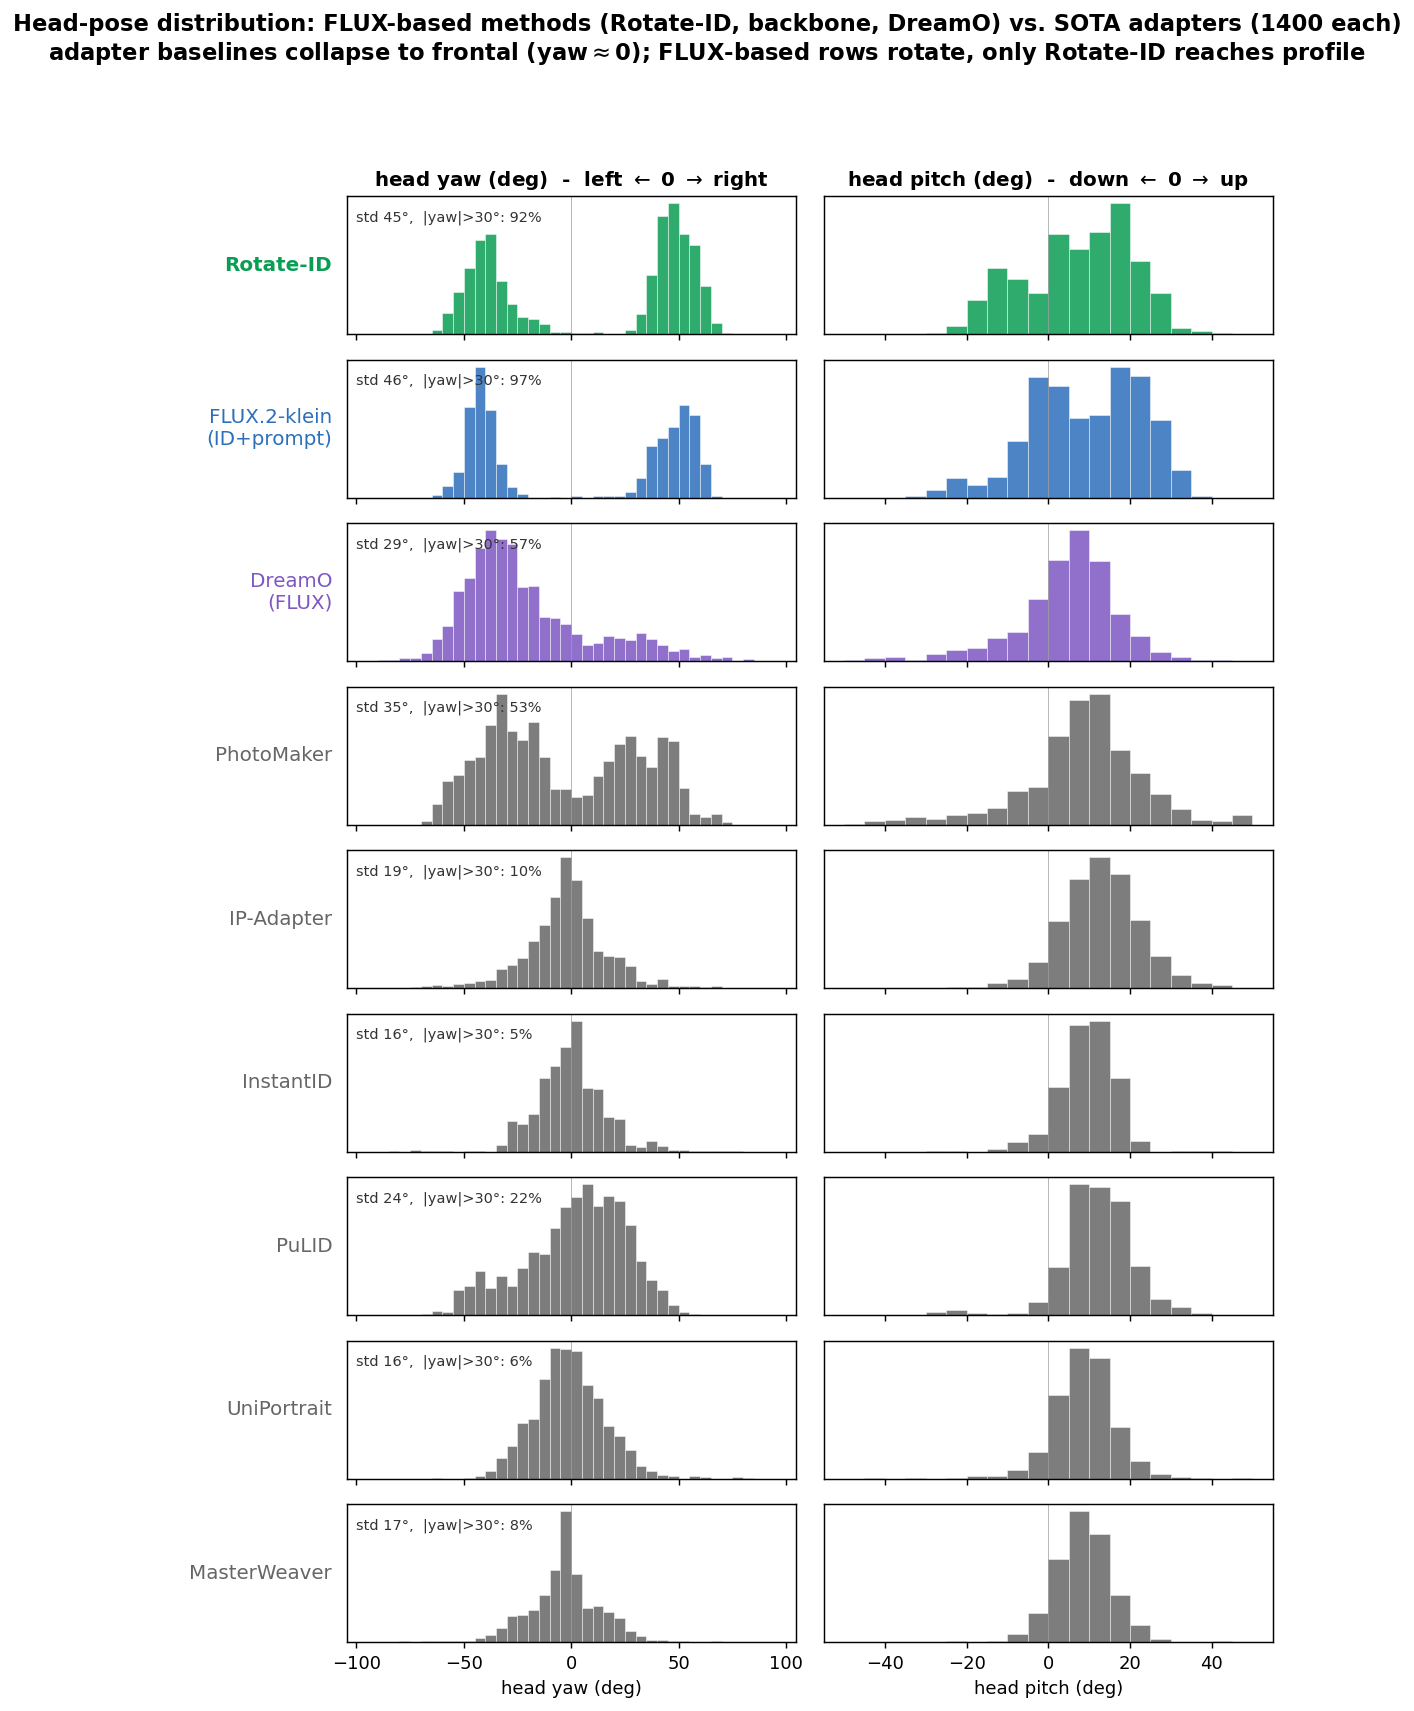
\includegraphics[width=\linewidth]{figures/pose_distribution.png}
\caption[Head-pose distribution]{\textbf{Head-pose distribution}: the three FLUX-based methods (Rotate-ID,
the FLUX.2-klein backbone, and DreamO~\cite{dreamo}) vs.\ six SD-adapter baselines
($1400$ generations each). The FLUX-based rows produce wide, off-frontal yaw
distributions ($|\theta_y|{>}30^\circ$ for $92\%$, $97\%$, and $57\%$ of faces),
whereas the SD adapters stay frontal-dominated (PhotoMaker the only one that
spreads appreciably). Crucially, \emph{only} Rotate-ID reaches the profile regime:
the in-context FLUX substrate enables rotation, and our structural control pushes
it to large angles. Pitch stays mostly chin-\emph{up}, the chin-down axis no
backbone reaches. The same breakdown per individual method is
App.~\ref{sec:appendix_thresh}.}
\label{fig:posedist}
\end{figure}

\FloatBarrier
\section{Identity under pose}
\label{sec:exp_id}
Sec.~\ref{sec:exp_setup} showed Rotate-ID rotates most reliably and flagged the
baselines' raw identity lead as a frontal-bias artifact; this section asks how
much of that gap is the \emph{recognizer's} bias specifically, and how much is
identity Rotate-ID itself has to earn. Two observations, one per question.
First, the pose-robust \emph{PAEs} score is consistently higher than overall
AdaFace (Rotate-ID $0.377$ vs.\ $0.297$; Table~\ref{tab:sota_pose}): the
angle-matched expert still finds the identity, and a \emph{single} cross-pose
encoder ($E_{fs}$ or $E_{fp}$) applied to all images matches the routed PAEs
to within $\sim\!0.04$, so this recovery reflects the pose-adapted encoders
themselves, not the bin-selection rule---confirming the recognizer-artifact
reading is real, not a metric-design coincidence. Second, independent of which
encoder reads it, Rotate-ID builds this identity from the bare backbone with
no prompt edit: Table~\ref{tab:id_bins} isolates the contribution of each
component, and we return to it as the formal component ablation in
Sec.~\ref{sec:exp_ablate}.

\noindent\textbf{Takeaway.} \emph{The recognizer-artifact reading holds up
under independent pose-adapted encoders, not just PAEs' own bin rule---and the
identity Rotate-ID recovers on top of that is earned with no prompt edit,
purely by reallocating attention to the reference.}

\begin{table}[t]\centering\small
\setlength{\tabcolsep}{5pt}
\adjustbox{max width=\linewidth}{%
\begin{tabular}{l cc @{\hskip 8pt} cc}
\toprule
\multirow{2}{*}{Configuration} & \multicolumn{2}{c}{raw CSIM} & \multicolumn{2}{c}{pose-aware ($k{=}4$)} \\
\cmidrule(lr){2-3}\cmidrule(lr){4-5}
 & Ada & PAEs & Ada & PAEs \\
\midrule
ID\,+\,prompt, no skeleton & 0.135 & 0.227 & 0.047 & 0.079 \\
\midrule
\dupid{}/m & 0.270 & 0.362 & 0.136 & 0.183 \\
\textbf{Rotate-ID} (\dupid{}\,+\,gate) & \textbf{0.297} & \textbf{0.377} & \textbf{0.148} & \textbf{0.188} \\
\bottomrule
\end{tabular}}
\caption[Identity ablation]{\textbf{Identity ablation} ($1400$ generations): mean AdaFace and PAEs CSIM
over detected faces, \emph{raw} and \emph{pose-aware}
$\widetilde{\mathrm{CSIM}}{=}\mathrm{CSIM}\cdot e^{-4P_e}$ at $k{=}4$
(Eq.~\ref{eq:posepenalty}). From the naive FLUX.2 base (identity image\,+\,prompt,
no structural control), \dupid{} and the learned gate recover identity
\emph{purely by reallocating attention to the reference}---no prompt edit. All three
configurations rotate comparably ($73.6$--$82.9\%$ yaw), so the gains persist under
the pose-aware discount.}
\label{tab:id_bins}
\end{table}

\FloatBarrier
\section{Pose-aware identity: sweeping the penalty $k$}
\label{sec:exp_penalized}
Secs.~\ref{sec:exp_setup}--\ref{sec:exp_id} established \emph{that} the
baselines' identity lead is a frontal-bias artifact; this section turns that
qualitative reading into a single tunable number, so the claim does not rest
on one arbitrarily-chosen discount strength. Recall from Sec.~\ref{sec:metrics}
the \emph{pose-aware identity}
$\widetilde{\mathrm{CSIM}}(k)=\mathrm{CSIM}\cdot e^{-k P_e}$
(Eq.~\ref{eq:posepenalty}): it discounts each method's mean AdaFace (or PAEs)
\csim{} by its yaw error $P_e{=}1-\mathrm{Acc_{yaw}}$, with $k{=}0$ the raw mean and
larger $k$ punishing unrealized rotation more. We now sweep $k$ itself, rather
than fixing it, to check the ranking is not an artifact of the $k{=}4$ chosen
elsewhere in this chapter.

Table~\ref{tab:posepenalized} reports the raw means and the pose-aware identity at
$k{=}4$; Fig.~\ref{fig:posepenalized} sweeps $k$. At $k{=}0$ (raw) the
frontal-collapsing baselines lead (InstantID $0.743$ AdaFace, $0.688$ PAEs) and
\textbf{Rotate-ID} sits mid-pack---exactly the artifact this paper warns about. But
those baselines almost never realize the rotation ($P_e\,{\gtrsim}\,0.6$, up to
$0.94$), so the penalty compounds against them: Rotate-ID ($P_e{=}0.17$) overtakes
\emph{every} baseline at $k\,{\gtrsim}\,1.7$ for AdaFace ($k\,{\gtrsim}\,1.0$ for
PAEs), and by $k{=}4$ leads on \emph{both} encoders ($0.148$ AdaFace, $0.188$ PAEs)
by a wide margin. The gap holds even against \textbf{DreamBooth}$^\dagger$, which
fine-tunes the backbone \emph{per identity}: despite the highest \emph{raw} identity
of any rotating method, it rotates less reliably (yaw $66.7$ vs.\ $82.6$), so the
yaw penalty discounts it more and it falls behind Rotate-ID ($0.085$ vs.\ $0.148$
AdaFace at $k{=}4$). Rotate-ID thus \emph{surpasses even a test-time-fine-tuning
baseline once rotation is credited}, while remaining the strongest tuning-free
one-shot method.

\noindent\textbf{Takeaway.} \emph{Sweep the penalty $k$ and every
frontal-collapsing baseline falls away by $k\!\approx\!1.7$; Rotate-ID leads on
both encoders at $k{=}4$, including over per-identity fine-tuning.}

\begin{table}[t]\centering\small
\setlength{\tabcolsep}{4pt}
\adjustbox{max width=\linewidth}{%
\begin{tabular}{ll c @{\hskip 6pt} cc @{\hskip 8pt} cc}
\toprule
\multirow{2}{*}{Method} & \multirow{2}{*}{Type} & \multirow{2}{*}{s/img} & \multicolumn{2}{c}{raw CSIM} & \multicolumn{2}{c}{pose-aware ($k{=}4$)} \\
\cmidrule(lr){4-5}\cmidrule(lr){6-7}
 & & & Ada & PAEs & Ada & PAEs \\
\midrule
\textbf{Rotate-ID (ours)} & ours & 10.1 & 0.297 & 0.377 & \textbf{0.148} & \textbf{0.188} \\
\midrule
DreamBooth$^\dagger$~\cite{dreambooth} & fine-tuning & 1.3 & 0.323 & 0.379 & 0.085 & 0.100 \\
\midrule
UNO~\cite{uno} & \multirow{2}{*}{adapter} & 14.5 & 0.226 & 0.358 & 0.011 & 0.018 \\
IP-Adapter~\cite{ipadapter} & & 3.6 & 0.537 & 0.541 & 0.017 & 0.017 \\
\midrule
PhotoMaker-V2~\cite{photomaker} & \multirow{7}{*}{encoder} & 5.6 & 0.454 & 0.505 & 0.035 & 0.039 \\
DreamO~\cite{dreamo} & & 15.0 & 0.560 & 0.619 & 0.040 & 0.044 \\
MasterWeaver~\cite{masterweaver} & & 1.2 & 0.313 & 0.483 & 0.009 & 0.014 \\
UniPortrait~\cite{uniportrait} & & 0.9 & 0.464 & 0.566 & 0.012 & 0.015 \\
PuLID~\cite{pulid} & & 3.3 & 0.553 & 0.631 & 0.014 & 0.016 \\
InstantID~\cite{instantid} & & 6.3 & \textbf{0.743} & \textbf{0.688} & 0.019 & 0.018 \\
WithAnyone~\cite{withanyone} & & 13.5 & 0.468 & 0.526 & 0.011 & 0.012 \\
\midrule
Step1X-Edit~\cite{step1xedit} & \multirow{2}{*}{image-edit} & 13.1 & 0.490 & 0.541 & 0.014 & 0.016 \\
OmniGen2~\cite{omnigen2} & & 9.0 & 0.308 & 0.402 & 0.033 & 0.043 \\
\bottomrule
\end{tabular}}
\caption[Pose-aware identity]{\textbf{Pose-aware identity}, grouped by method \emph{type}: mean AdaFace
and PAEs CSIM (\emph{raw}) and the pose-aware
$\widetilde{\mathrm{CSIM}}{=}\mathrm{CSIM}\cdot e^{-4P_e}$ at $k{=}4$, with
$P_e{=}1-\mathrm{Acc_{yaw}}$ (Eq.~\ref{eq:posepenalty}; raw CSIM and yaw accuracy from
Table~\ref{tab:sota_pose}). Bold = best \emph{tuning-free}. The frontal-collapsing
baselines lead on \emph{raw} identity (InstantID) but earn it \emph{without
realizing the rotation}; once the yaw penalty applies ($k{=}4$), \textbf{Rotate-ID} is the
best method on \emph{both} encoders. $^\dagger$DreamBooth, despite higher \emph{raw}
identity, trails Rotate-ID here because it rotates less reliably ($66.7$ vs.\ $82.6\%$
yaw) and is penalized more---besides fine-tuning the backbone \emph{per identity}.}
\label{tab:posepenalized}
\end{table}

\begin{figure}[t]\centering
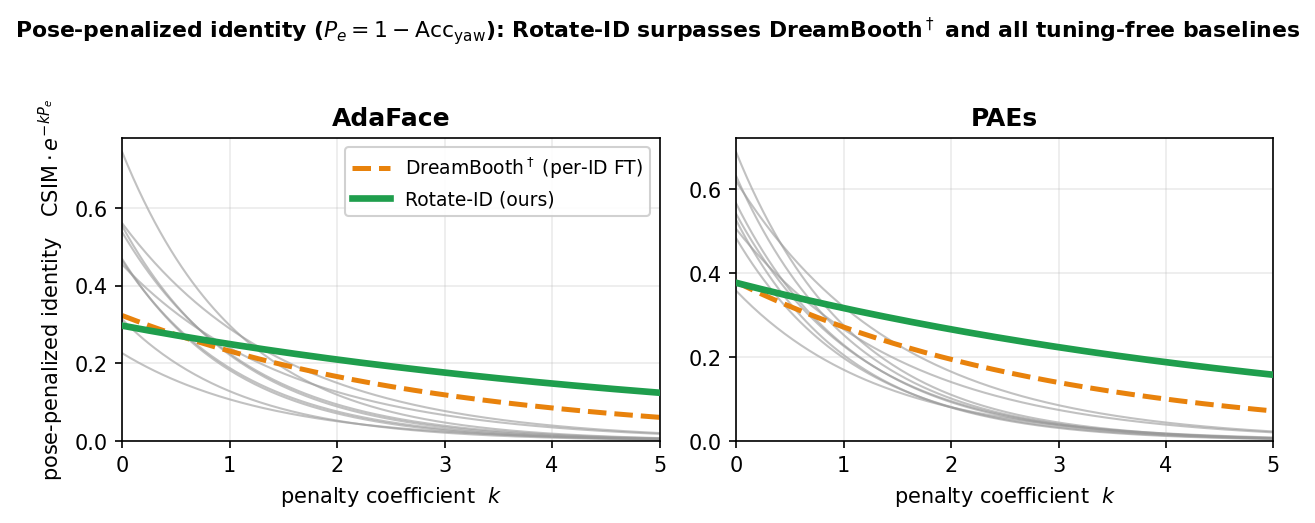
\includegraphics[width=\linewidth]{figures/pose_penalized.png}
\caption[Pose-aware identity vs.\ penalty $k$]{\textbf{Pose-aware identity vs.\ penalty $k$}
(Eq.~\ref{eq:posepenalty}, $P_e{=}1-\mathrm{Acc_{yaw}}$).
Tuning-free baselines (gray) start high but decay steeply---their identity is a
near-frontal artifact; \textbf{Rotate-ID} (green, $P_e{=}0.17$) stays nearly flat
and overtakes all of them at $k\,{\approx}\,1.7$ (AdaFace)\,/\,$1.0$ (PAEs).
\textbf{DreamBooth}$^\dagger$ (orange, per-identity fine-tuning) starts higher but,
rotating less, is overtaken as well.}
\label{fig:posepenalized}
\end{figure}

\FloatBarrier
\section{Ablation: the identity--pose trade-off}
\label{sec:exp_ablate}
Sec.~\ref{sec:exp_penalized} established \emph{that} Rotate-ID is the strongest
pose-aware method at every reasonable $k$; this section asks \emph{which part}
of the method earns that result. We ablate every mechanism-level design
decision of Secs.~\ref{sec:refgeometry}--\ref{sec:learned}: the presence of
each component, the duplication \emph{count}, the reference \emph{order}, and
the learned gate, each scored with the pose-rectified metrics of
Sec.~\ref{sec:metrics}.

\paragraph{Component ablation.}
Table~\ref{tab:id_bins} doubles as our identity ablation. Conditioning FLUX.2 on
the identity image and prompt \emph{alone}---no structural control---already rotates
the head ($73.6\%$ yaw) but at a near-total identity cost (AdaFace $0.135$, close to
the no-identity floor): the model renders the prompt's nominal person rather than
the reference (Fig.~\ref{fig:noskel}). Adding the structural control with reference
duplication (the \dupid{} winner) rotates just as well ($82.9\%$ yaw) and lifts
identity to $0.270$ AdaFace / $0.362$ PAEs. The \textbf{learned attention
gate}---the \textbf{Rotate-ID} configuration of Table~\ref{tab:sota_pose}---then
raises identity further to $0.297$ / $0.377$ while \emph{keeping} the full rotation
($82.6\%$ yaw), recovering identity purely by reallocating attention to the
reference, with no edit to the prompt. Because all three configurations rotate
comparably, the gain is not an artifact of trading pose for identity: under the
\emph{pose-aware} discount at $k{=}4$ the same ordering holds
($0.047\!\rightarrow\!0.136\!\rightarrow\!0.148$ AdaFace,
$0.079\!\rightarrow\!0.183\!\rightarrow\!0.188$ PAEs), so each component adds
identity \emph{without} giving up rotation---a controllable point on the
identity--pose Pareto. Figure~\ref{fig:teaser} shows the rotation-with-identity
result qualitatively.

\begin{figure}[t]\centering
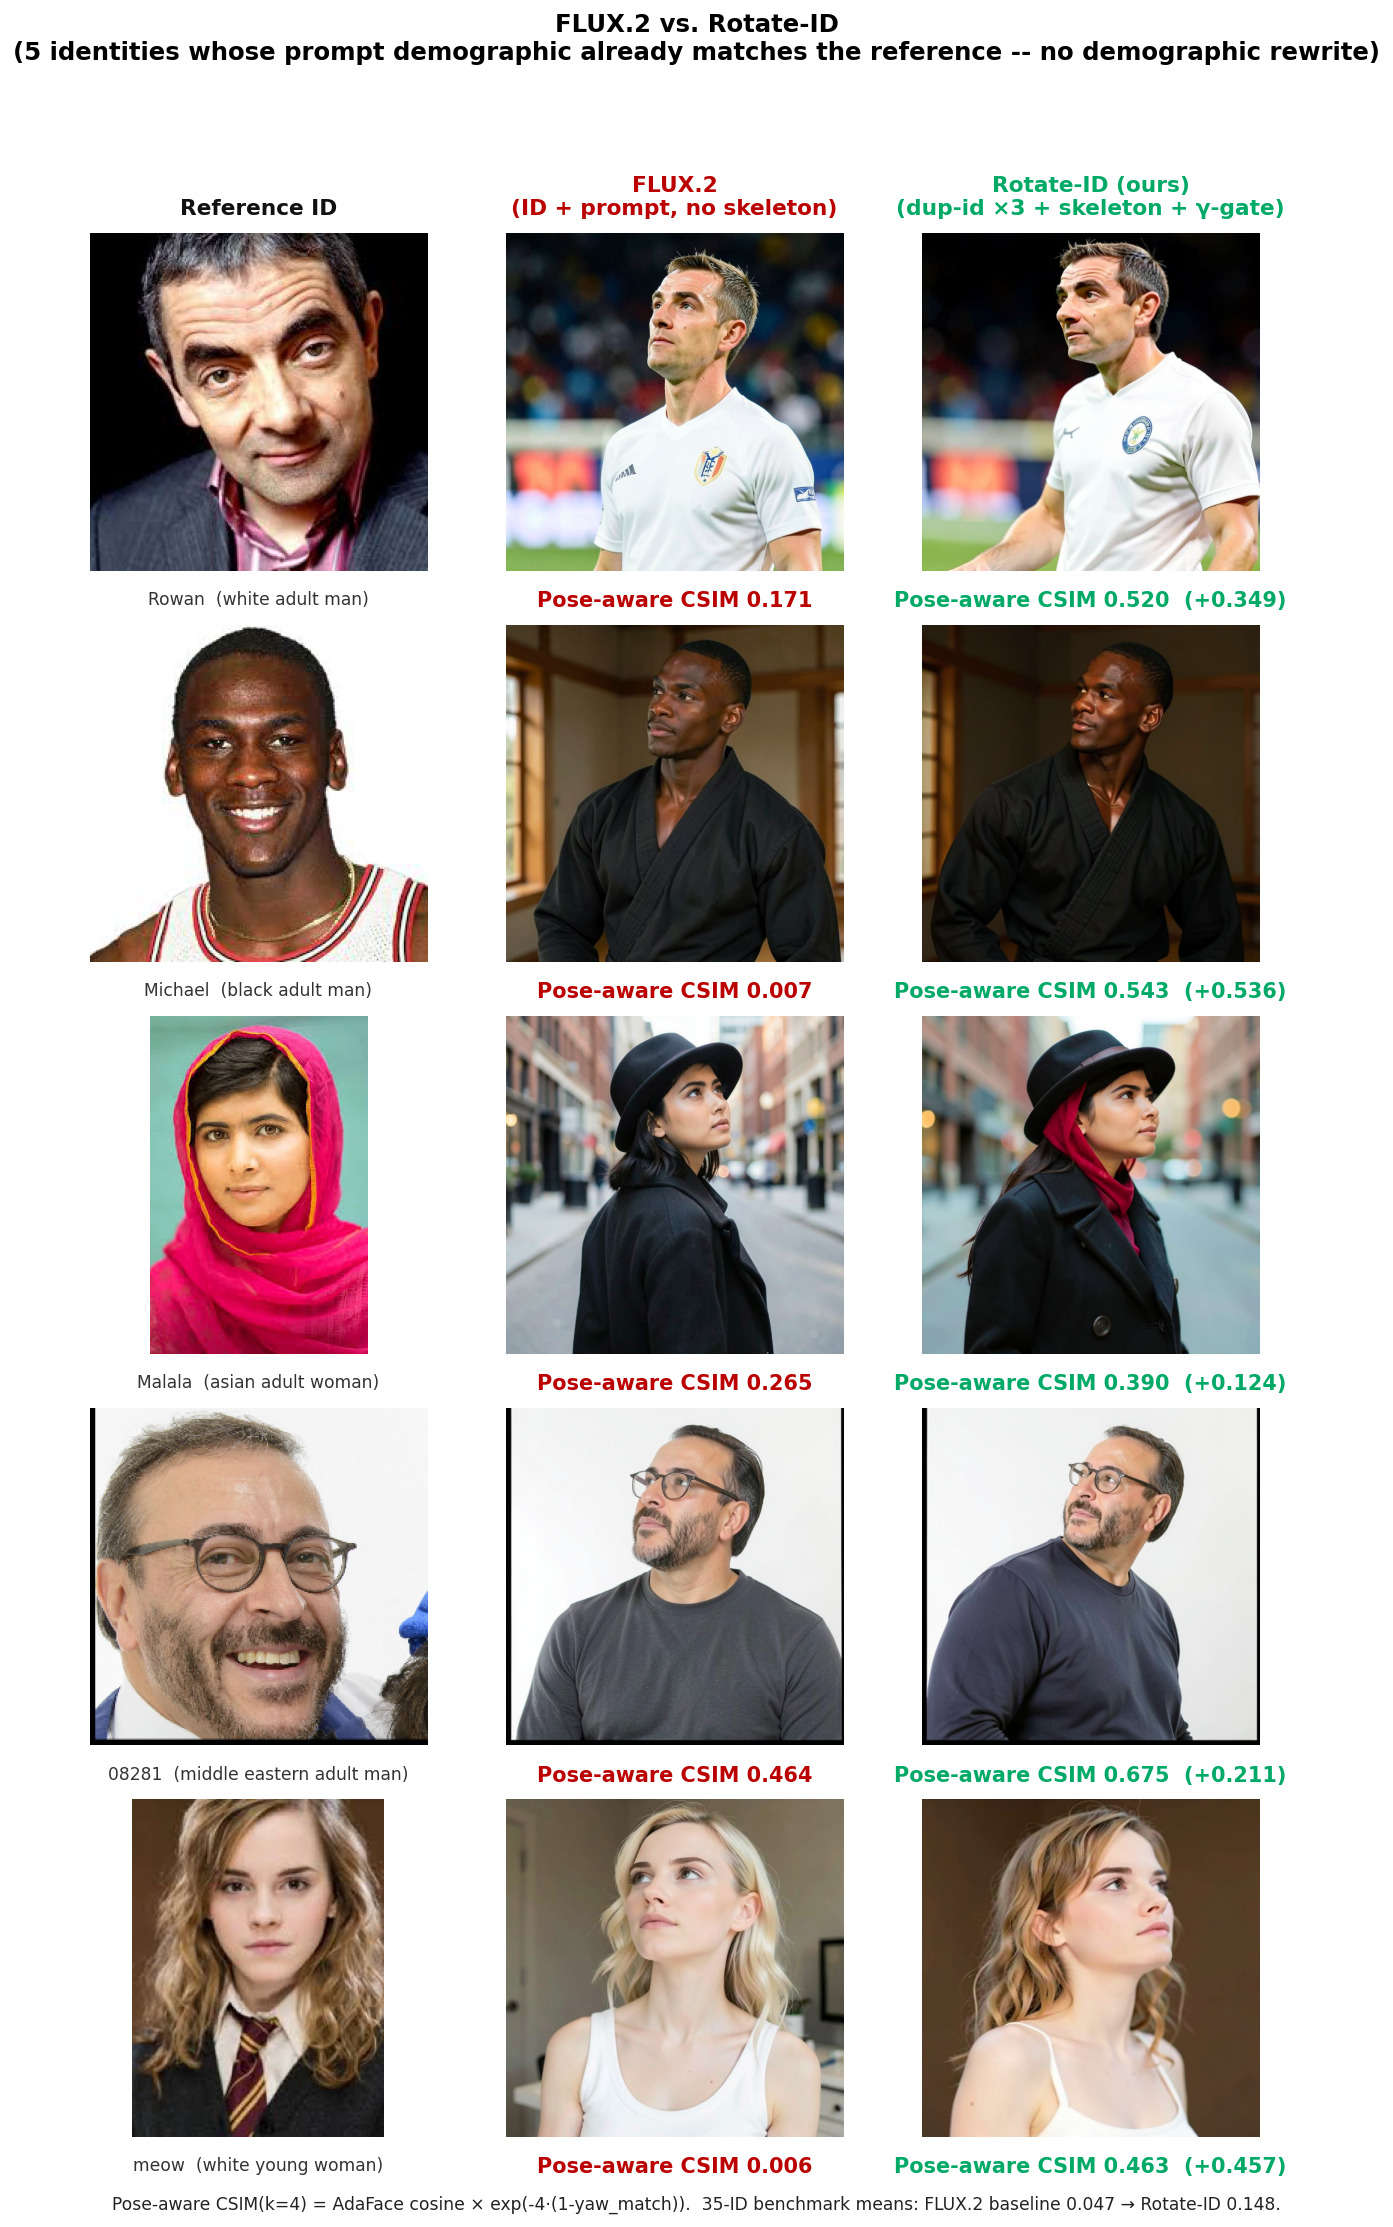
\includegraphics[width=0.75\linewidth]{figures/flux2_vs_rotateid_demomatch.png}
\caption[FLUX.2 vs.\ Rotate-ID on demographic-matched identities]{\textbf{FLUX.2 (identity + prompt, no skeleton) vs.\ Rotate-ID, on
identities whose prompt demographic already matches the reference} (no
demographic rewrite involved). Each row reports pose-aware \csim{} ($k{=}4$)
for FLUX.2 conditioned on the identity image and prompt alone and for the full
Rotate-ID (\dupid{} $\times 3$ + skeleton + \gate{}), with the gain annotated.
Without structural control, FLUX.2 already rotates from the prompt but drifts
toward the prompt's nominal person rather than the reference, costing
identity; Rotate-ID raises pose-aware \csim{} on every identity shown
($+0.124$ to $+0.457$). Across the full 35-identity benchmark the same
comparison averages $0.047\to 0.148$. This is the naive
baseline (top row of Table~\ref{tab:id_bins}) our components build on.}
\label{fig:noskel}
\end{figure}

\paragraph{Duplication count: identity saturates, pose pays.}
How far can duplication alone be pushed? We sweep $N\in\{1,2,3,4,5,6\}$ identity
copies at $170$ generation pairs per point ($17$ prompts $\times$ $10$
identities, benchmark configuration and seed), scoring each point with the full
pose-rectified pipeline (Fig.~\ref{fig:dupsweep170}). Raw identity rises
monotonically ($0.185\!\rightarrow\!0.539$ AdaFace) but pose pays a growing
price: pitch accuracy falls from $55.9\%$ to $24.1\%$ by $N{=}4$---the
over-weighted frontal reference flattens the chin---and yaw peaks at $N{=}3$
($78.8\%$) before sliding to $63.5\%$. The \emph{pose-aware} identity therefore
climbs only to $N{\approx}3$--$4$ ($0.156$/$0.161$) and folds thereafter. Pushed
further ($N{=}8,10$ on a smaller grid, Table~\ref{tab:dupsweep_full}), the
collapse is total: raw \csim{}
saturates at $0.97$ because the model \emph{copy-pastes} the reference---an
almost pixel-faithful frontal replica---while yaw accuracy falls to
$8$--$12\%$ and pitch to $0$. This answers the natural question ``why not more
copies, at higher compute?'': the bottleneck is the \emph{attention budget}, not
computation---extra identical blocks push the identity share toward $1$ and the
pose share toward $0$, buying recognizer similarity by abandoning the requested
posture. The \gate{} (star) attains a \emph{higher} pose-aware identity
($0.168$) than \emph{any} duplication count, at the sweep's best yaw
($78.8\%$)---duplication moves \emph{along} the identity--pose trade-off, the
learned gate moves \emph{off} it (Fig.~\ref{fig:dupPareto}).

\begin{table}[t]\centering\small
\setlength{\tabcolsep}{5pt}
\adjustbox{max width=\linewidth}{%
\begin{tabular}{lccc}
\toprule
Setting & Yaw acc & Pitch acc & pose-aware \csim{} ($k{=}4$) \\
\midrule
\multicolumn{4}{@{}l}{\emph{$170$-pair grid ($17$ prompts $\times$ $10$ identities)}} \\
\dupid{} $=1$ (single ref) & 72.4 & 55.9 & 0.061 \\
\dupid{} $\times 3$ & 78.8 & 42.4 & 0.156 \\
\textbf{\dupid{} $\times 3$ + \gate{}} & \textbf{78.8} & \textbf{42.4} & \textbf{0.168} \\
\midrule
\multicolumn{4}{@{}l}{\emph{Extended sweep ($6$ prompts $\times$ $5$ identities)}} \\
\dupid{} $=1$ & 65.4 & 53.8 & 0.046 \\
\dupid{} $=2$ & 53.3 & 40.0 & 0.057 \\
\dupid{} $=3$ & 69.2 & 34.6 & 0.114 \\
\dupid{} $=4$ & 66.7 & 29.2 & 0.130 \\
\dupid{} $=6$ & 45.8 & 12.5 & 0.076 \\
\dupid{} $=8$ & 8.3 & 0.0 & 0.025 \\
\dupid{} $=10$ & 12.5 & 0.0 & 0.029 \\
\textbf{\dupid{} $\times 3$ + \gate{}} & \textbf{73.1} & \textbf{34.6} & \textbf{0.143} \\
\midrule
\multicolumn{4}{@{}l}{\emph{Full $40$-prompt benchmark ($1400$ generations)}} \\
\dupid{} $\times 3$ (no gate) & 82.9 & 39.4 & 0.136 \\
\textbf{Rotate-ID (\dupid{} $\times 3$ + \gate{})} & \textbf{82.6} & \textbf{39.0} & \textbf{0.148} \\
\bottomrule
\end{tabular}}
\caption[Duplication-count sweep, every mechanism setting]{\textbf{Duplication-count sweep, every mechanism setting} (pose-rectified
metrics; yaw/pitch = direction accuracy). Three grids agree: the $170$-pair grid
anchors the $N{=}1$, $N{=}3$, and $N{=}3$+\gate{} points also swept continuously
in Fig.~\ref{fig:dupsweep170}; an extended sweep pushes duplication to $N{=}10$,
where pose collapses (yaw $\leq\!12.5\%$, pitch $0\%$) as the model copy-pastes
the reference (raw \csim{} saturates near $0.97$); and the full $1400$-generation
benchmark confirms the same ordering at scale. \dupid{} $\times\,3$+\gate{} is
the best joint yaw/pitch/pose-aware operating point in every grid.}
\label{tab:dupsweep_full}
\end{table}

\begin{figure}[t]\centering
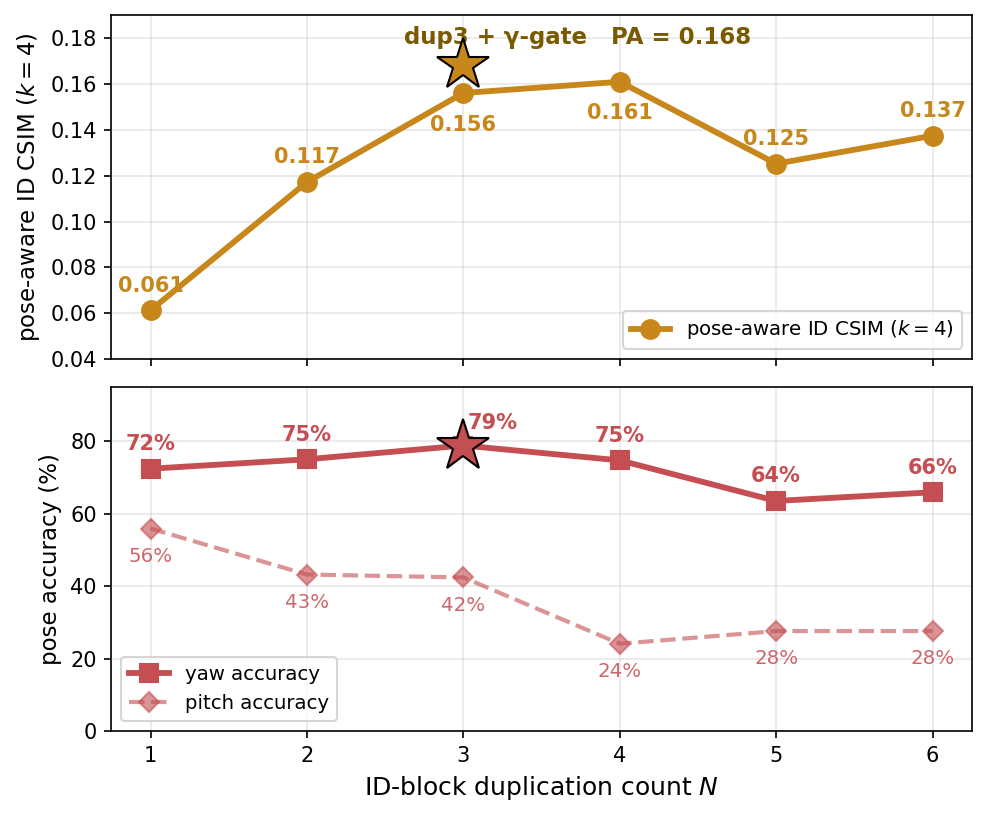
\includegraphics[width=\linewidth]{figures/mech_dup170_sweep.png}
\caption[Duplication-count sweep at scale]{\textbf{Duplication-count sweep at scale} ($170$ pairs/point,
pose-rectified metrics; benchmark configuration, fixed seed). Pose-aware identity
(gold) climbs steadily to its $N{\approx}3$ operating point while pose pays a
growing price (pitch, dashed, halves by $N{=}4$; yaw falls after $N{=}3$). The
\gate{} ($\star$) lifts pose-aware identity above \emph{every} duplication count
at no pose cost.}
\label{fig:dupsweep170}
\end{figure}

\begin{figure}[t]\centering
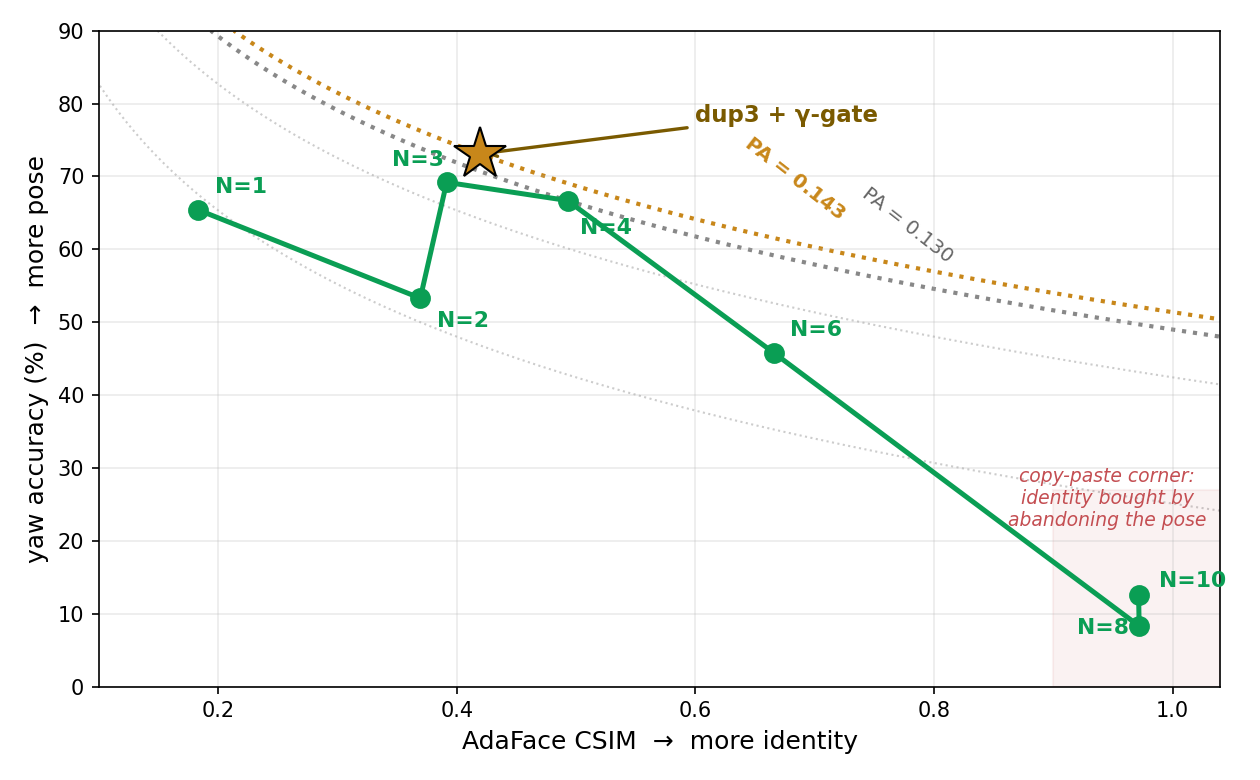
\includegraphics[width=\linewidth]{figures/mech_dupN_pareto.png}
\caption[The identity--pose Pareto view of duplication]{\textbf{The identity--pose Pareto view of duplication.} Each point is a
duplication count (paper-aligned metrics); dotted curves are iso-contours of the
pose-aware identity ($k{=}4$). Duplication only \emph{trades along} the curve---at
$N{\ge}6$ it slides into the copy-paste corner (near-perfect \csim{}, pose
abandoned)---whereas the \gate{} ($\star$) is the only point on the highest
pose-aware contour: it moves \emph{off} the trade-off rather than along it.}
\label{fig:dupPareto}
\end{figure}

\FloatBarrier
\paragraph{What the gate learned.}
Fig.~\ref{fig:gateschedule} inspects the trained allocator itself. Averaged over
layers, the identity gain follows a \emph{late-step} schedule---$\gamma_{\mathrm{id}}
\approx[1.00,1.05,1.06,1.22]$ across the four denoise steps---leaving the early
structure-setting steps untouched (where the skeleton lays out the pose) and
boosting identity where facial detail is refined; the frozen skeleton gain
($\gamma_{\mathrm{skel}}{=}1$) confirms no pose channel was touched. This learned
schedule is why the gate adds identity at \emph{no} pose cost in every table of
this section: it re-allocates the budget only when and where identity is cheap
to buy.

\begin{figure}[t]\centering
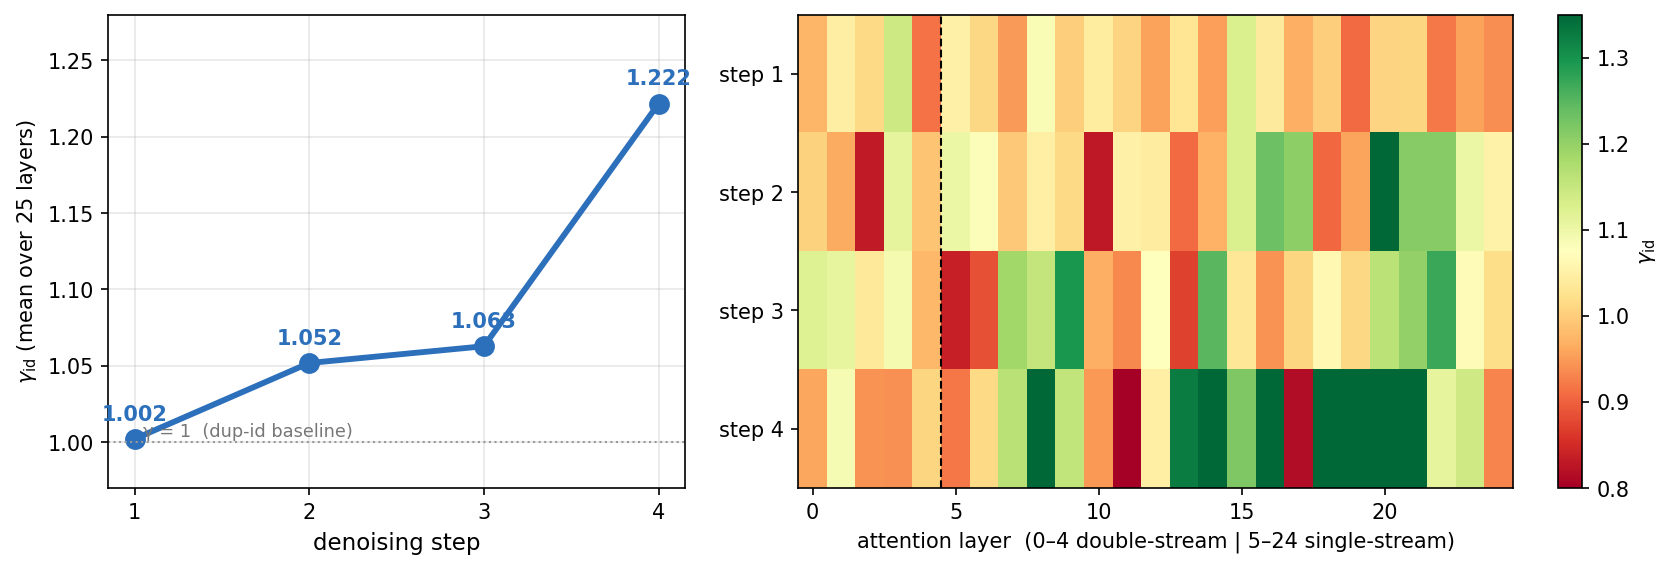
\includegraphics[width=\linewidth]{figures/mech_gate_schedule.png}
\caption[The learned allocator's schedule]{\textbf{The learned allocator's schedule.} Left: per-step identity gain
$\gamma_{\mathrm{id}}$ (mean over the $25$ layers) rises only at the late,
detail-refining steps ($+22\%$ at the final step). Right: the full
$(\text{step},\text{layer})$ gain map of the $\sim$200-parameter tensor; the
skeleton gain is frozen at $1$. The gate buys identity exactly where it does not
compete with pose formation.}
\label{fig:gateschedule}
\end{figure}

\FloatBarrier
\paragraph{Qualitative view.}
Fig.~\ref{fig:visualprogress} traces one prompt/seed across every setting: with a
single reference the model renders a \emph{different person}; identity emerges by
$N{=}3$; the gate refines it; and at $N{\ge}8$ the output degenerates into a
pasted copy of the reference with the requested posture ignored---the visual
counterpart of the curves above.

\noindent\textbf{Takeaway.} \emph{Each component adds identity without giving up
rotation; duplication only trades along the identity--pose curve, and the
$\sim$200-parameter \gate{} is the only setting that moves above it.}

\begin{figure}[t]\centering
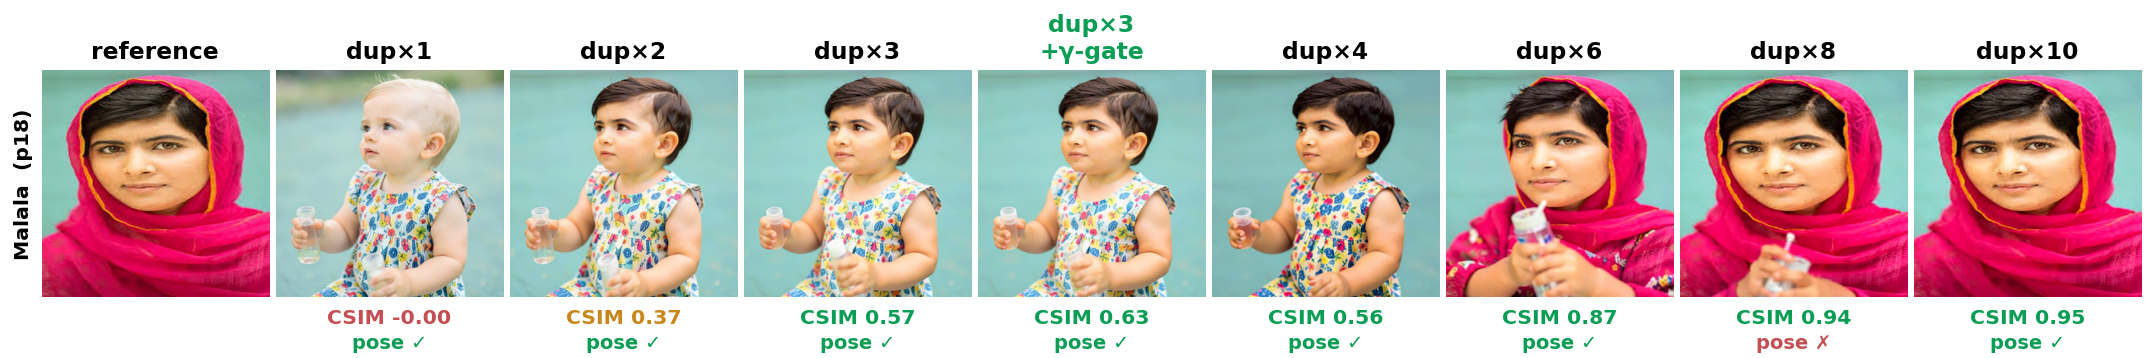
\includegraphics[width=\textwidth]{figures/mech_visual_settings_progression_single.png}
\caption[Every setting, one prompt and seed, to the copy-paste endpoint]{\textbf{Every setting, one prompt and seed, to the copy-paste endpoint}
(full frames; AdaFace \csim{} and pose verdict under each image)---the
\emph{Malala} row of Fig.~\ref{fig:idemergence}, extended past $N{=}6$ to the
two duplication counts that chapter stopped short of. The $N{\le}6$ cells
repeat what Fig.~\ref{fig:idemergence} already showed (identity lost at
$N{=}1$, recovered by $N{=}3$, refined by the \gate{}); the new information is
what happens if duplication is pushed further: $N{\ge}8$ collapses into
copy-paste---near-perfect \csim{} with the posture request abandoned
(\emph{pose}~\xmark).}
\label{fig:visualprogress}
\end{figure}
